\documentclass{article}
\usepackage[utf8]{inputenc}
\usepackage{blindtext}
\usepackage{graphicx}
\usepackage{amsmath}
\usepackage{csvsimple}
\usepackage{pdfpages}
\usepackage{hyperref}
\usepackage{caption}
\usepackage{subcaption}

\title{Kapitán Brown}
\author{Martin Skok}

\begin{document}
\maketitle

\begin{abstract}
  Opilý kapitán Brown jde z hospody v 1D rovině (nikdy jsem nepsal abstrakt)
\end{abstract}

\section{Zadání}
Kapitán Brown vyjde v čase t = 0 z hospody v x = 0 a v každém kroku se s
pravděpodobností ½ přemístí o jeden krok vlevo nebo vpravo.
Zvolte vhodnou délku procházky tmax a počet opakování N pro získání statisticky
spolehlivých výsledků.\\
\newpage
\section{Data}
Jako první jsem nasimuloval náhodnou procházku v 1D. Použil jsem $t_{max} = 1000$
a $N = 1000$, kde $t_{max}$ je vlastně čas neboli dékla procházky a $N$ je počet procházek celkem.
Protože se data zdála nedostatečná, navýšil jsem počet opakování na $N = 10000$

\begin{figure}[hbt!]
  \begin{center}
    \includegraphics[scale=0.7]{walks.pdf}
    \end{center}
  \caption{Simulace náhodných procházek}
\end{figure}
\newpage

Poté jsem měl určit křivku $<x^{2} (t)>$.
Určil jsem ji tak, že jsem udělal průměr všech křivek na druhou mocninu.

\begin{figure}[hbt!]
  \begin{center}
    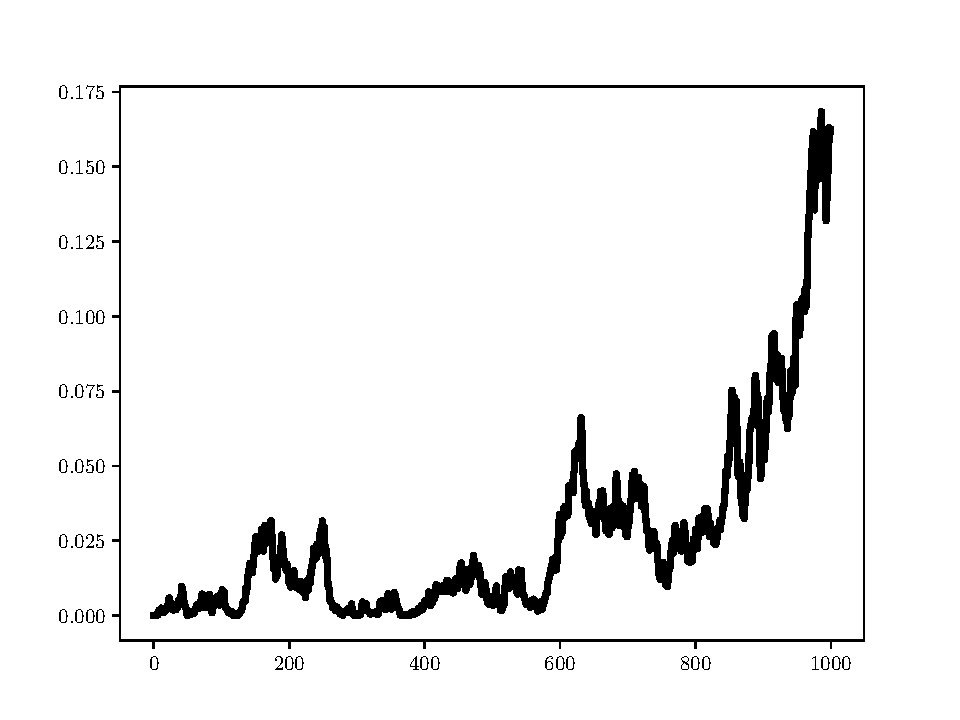
\includegraphics[scale=0.7]{walks2.pdf}
    \end{center}
  \caption{Křivka $<x^{2} (t)>$}
\end{figure}


\newpage
\section{Data}
Dále jsem si měl vybrat různé časové intervali a udělat v těchto časech historogramy.
Vybral jsem tedy 12 náhodných intervalů mezi $t_{i} \in [300, 10000]$.\\
Historogramy jsem nemusel normovat manuálně, program to udělal za mě, jak je popsáno v kodu.
To jsem potom fitnul normálovou distribucí, která je popsaná
$$f(t_{i}) = \frac{1}{\sqrt{2 \pi \sigma^{2}}} \cdot exp\left(-\frac{(t_{i} - \mu)^{2}}{2\sigma^{2}}\right)$$
$\sigma$ a $\mu$ program našel za mě taky.

\begin{figure}
\begin{subfigure}{.3\textwidth}
  \centering
  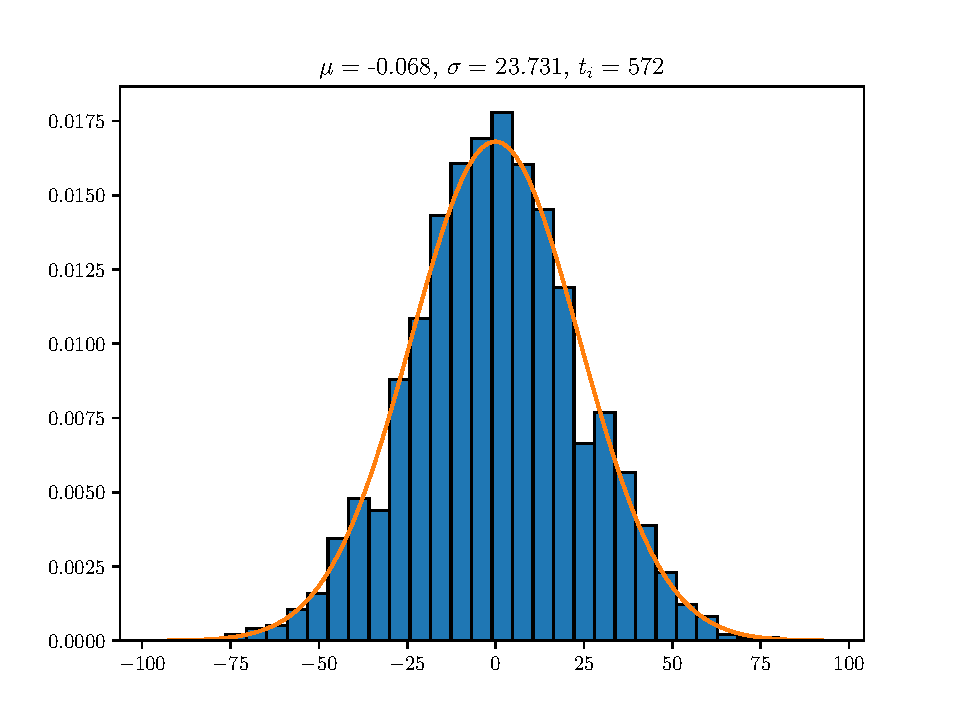
\includegraphics[width=1.1\linewidth]{hist1.pdf}
\end{subfigure}
\begin{subfigure}{.3\textwidth}
  \centering
  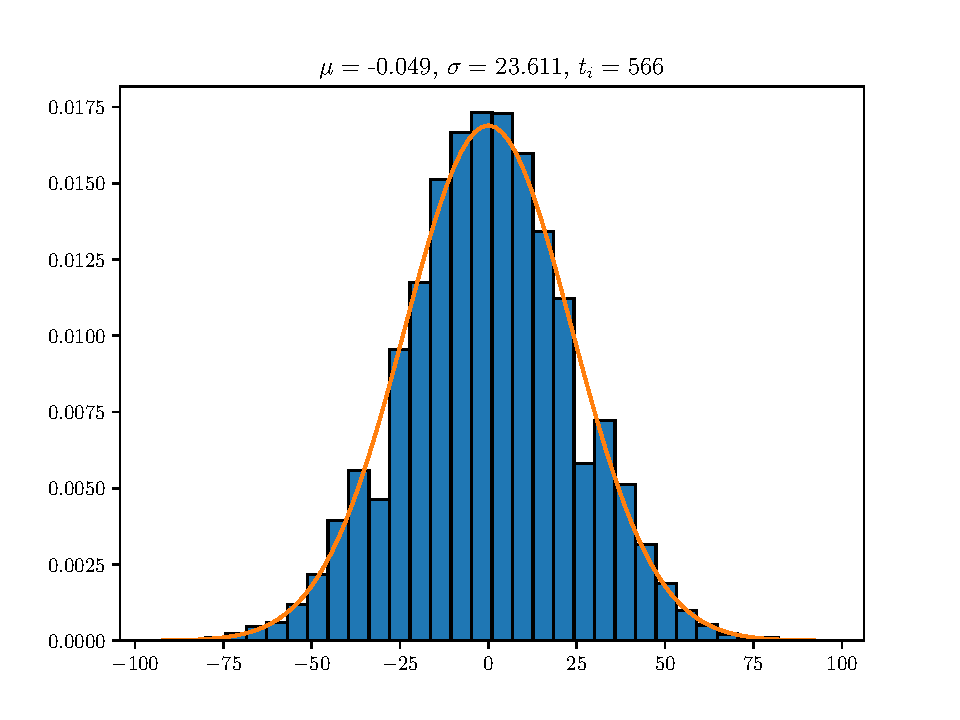
\includegraphics[width=1.1\linewidth]{hist2.pdf}
\end{subfigure}
\begin{subfigure}{.3\textwidth}
  \centering
  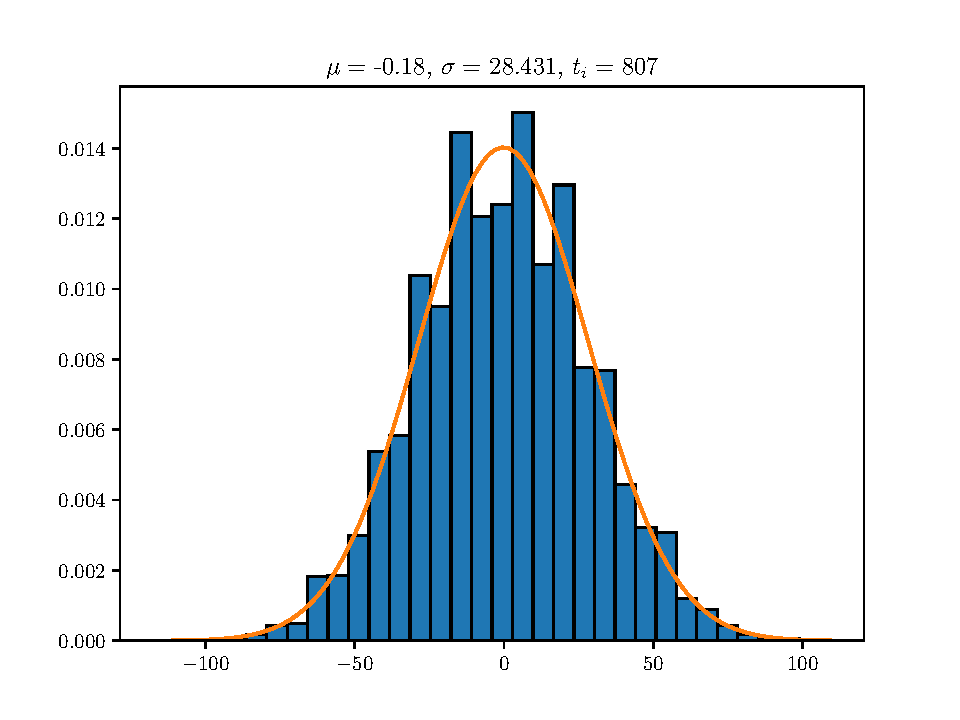
\includegraphics[width=1.1\linewidth]{hist3.pdf}
\end{subfigure}
\newline

\begin{subfigure}{.3\textwidth}
  \centering
  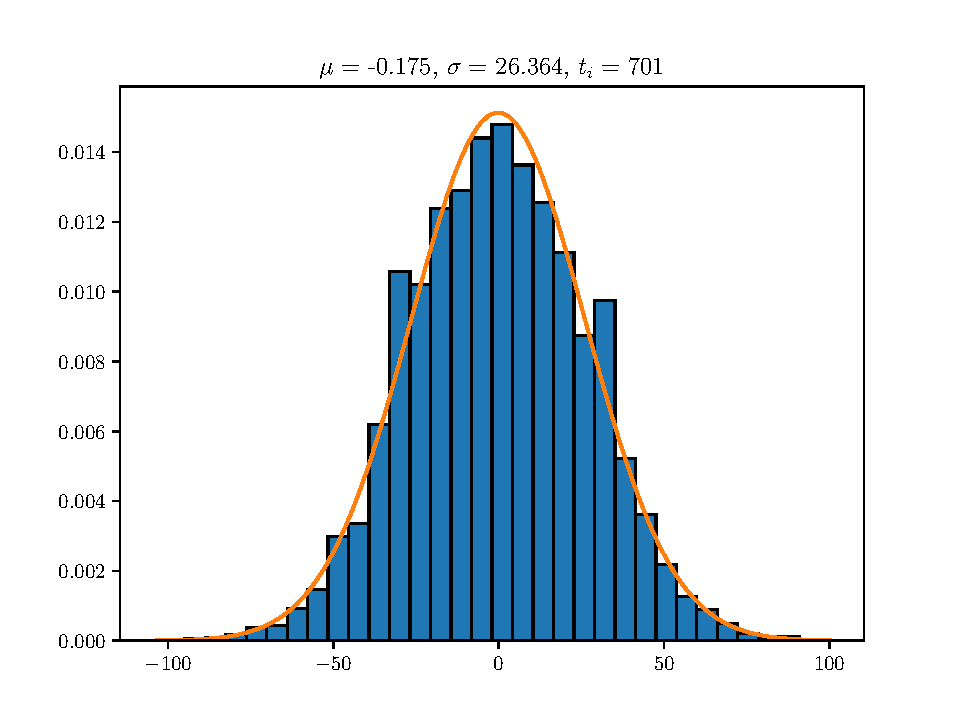
\includegraphics[width=1.1\linewidth]{hist4.pdf}
\end{subfigure}
\begin{subfigure}{.3\textwidth}
  \centering
  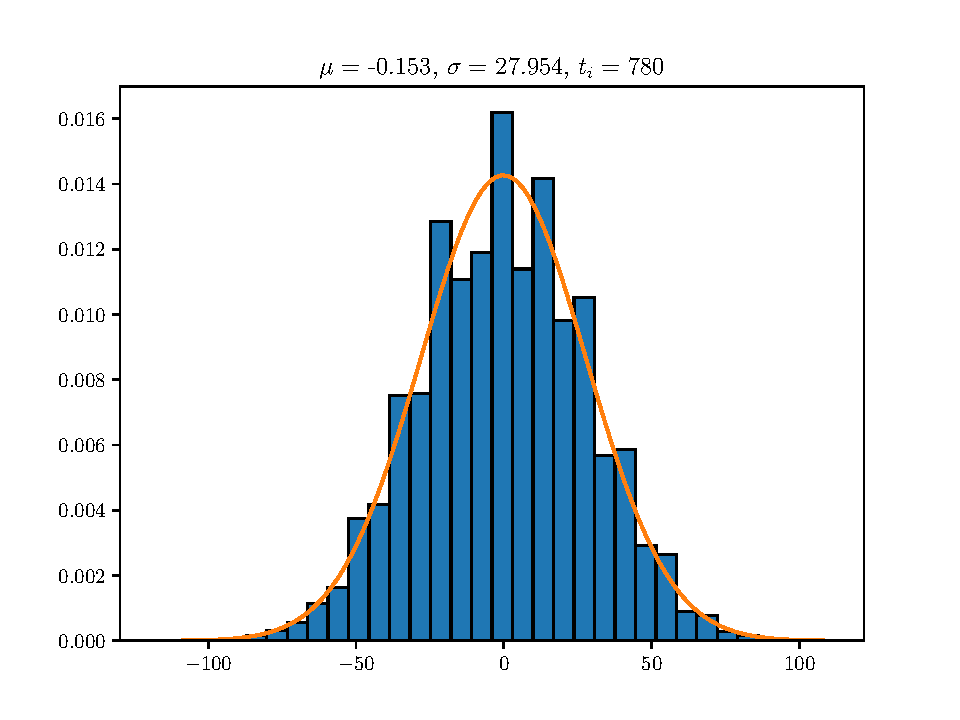
\includegraphics[width=1.1\linewidth]{hist5.pdf}
\end{subfigure}
\begin{subfigure}{.3\textwidth}
  \centering
  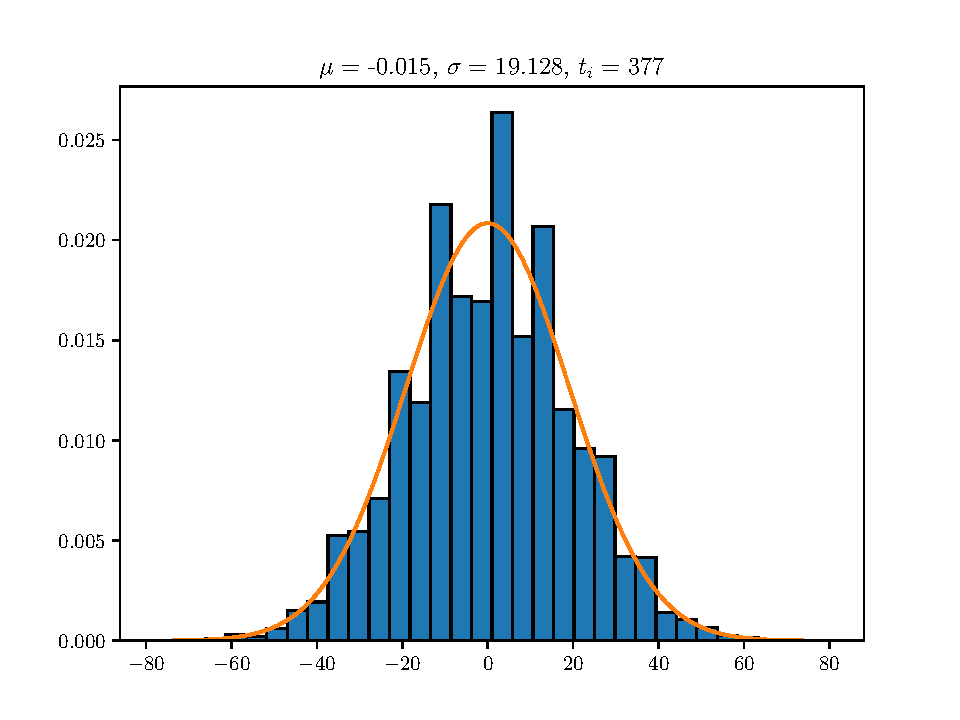
\includegraphics[width=1.1\linewidth]{hist6.pdf}
\end{subfigure}
\newline

\begin{subfigure}{.3\textwidth}
  \centering
  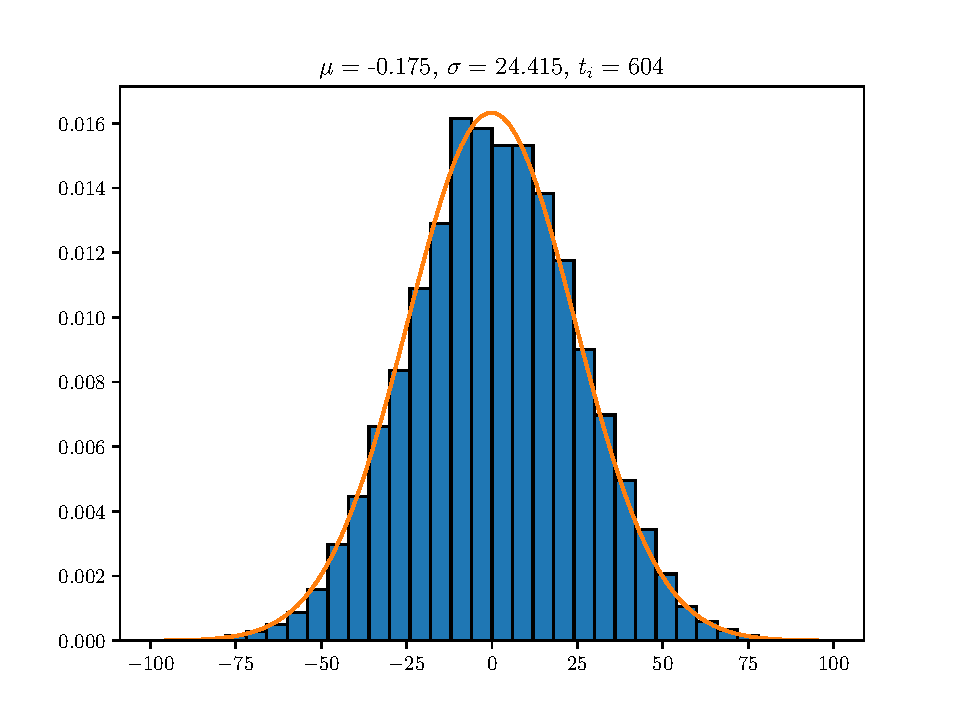
\includegraphics[width=1.1\linewidth]{hist7.pdf}
\end{subfigure}
\begin{subfigure}{.3\textwidth}
  \centering
  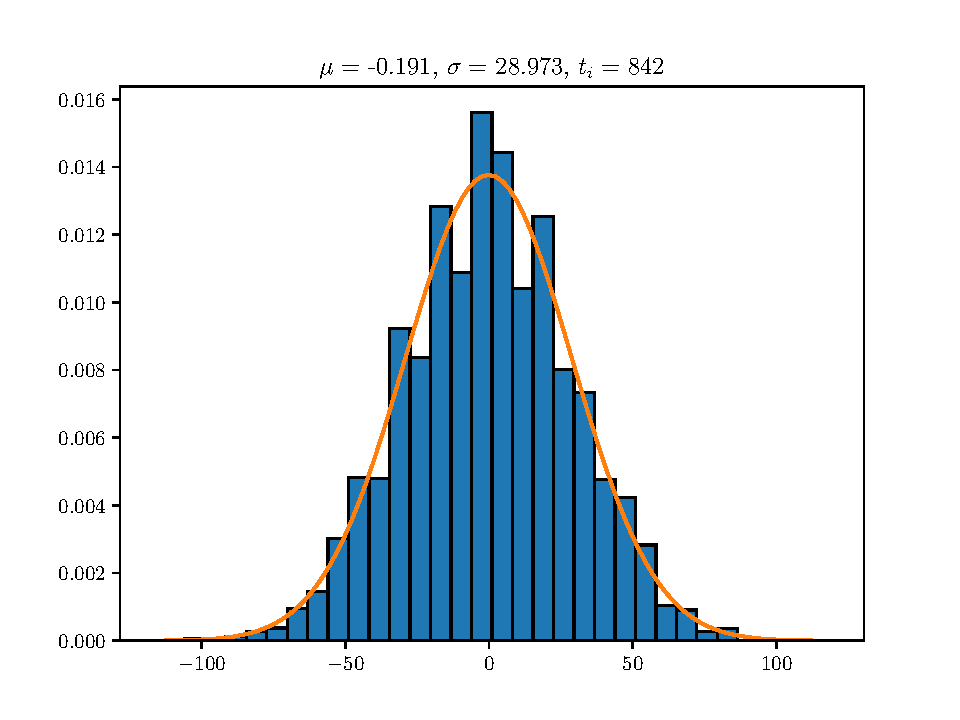
\includegraphics[width=1.1\linewidth]{hist8.pdf}
\end{subfigure}
\begin{subfigure}{.3\textwidth}
  \centering
  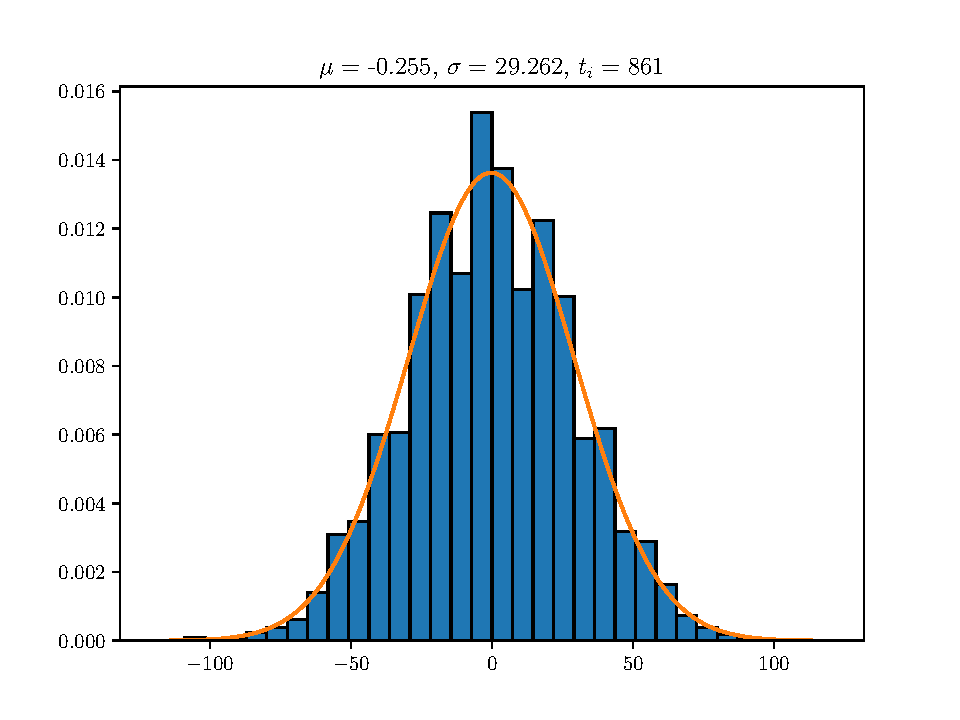
\includegraphics[width=1.1\linewidth]{hist9.pdf}
\end{subfigure}
\newline

\begin{subfigure}{.3\textwidth}
  \centering
  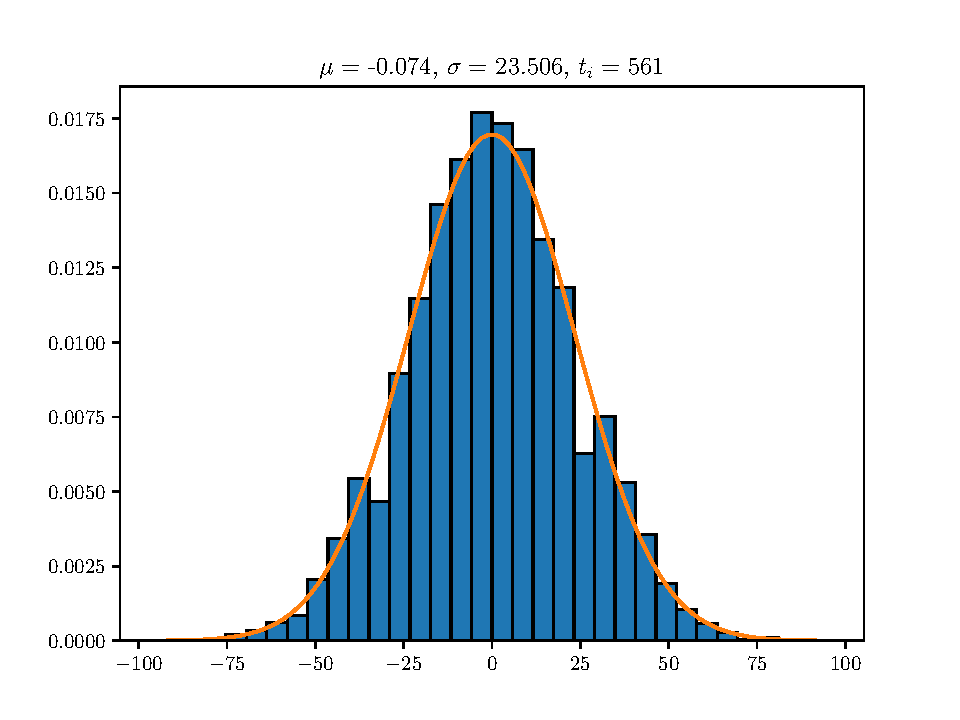
\includegraphics[width=1.1\linewidth]{hist10.pdf}
\end{subfigure}
\begin{subfigure}{.3\textwidth}
  \centering
  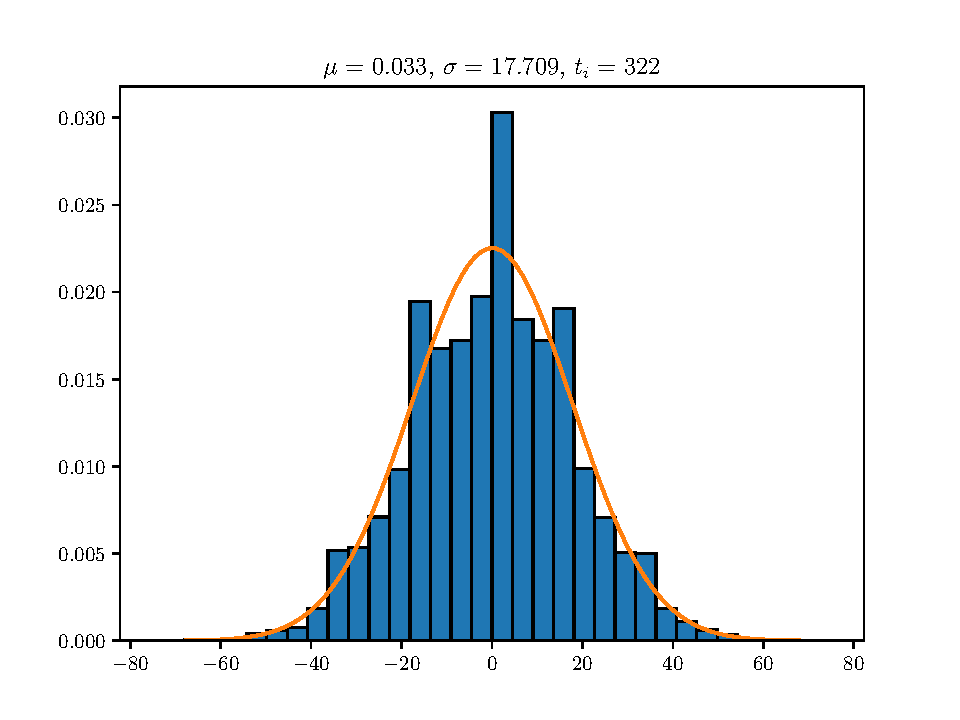
\includegraphics[width=1.1\linewidth]{hist11.pdf}
\end{subfigure}
\begin{subfigure}{.3\textwidth}
  \centering
  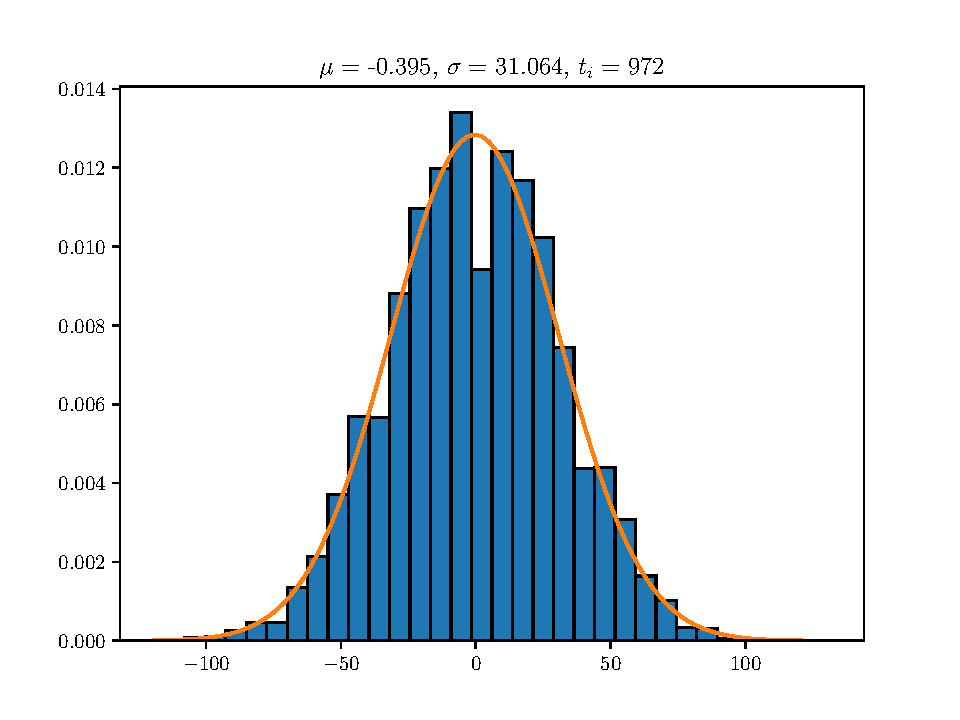
\includegraphics[width=1.1\linewidth]{hist12.pdf}
\end{subfigure}
\newline

\caption{Grafy ukazující hustotu pravděpodobnosti výskytu procházky}
\end{figure}

\newpage
Abych určil závislost $\sigma$ na $t_{i}$, vytvořil jsem tabulku.
Tabulka není řádně seřazena, protože jsem hodnoty generoval náhodně,
takže líp je to vidět až na grafu.

\begin{table}[!ht]
    \centering
    \begin{tabular}{|l|l|l|}
    \hline
        $t_{i}$ & $\mu$ & $\sigma$ \\ \hline
        351.0 & 0.21 & 18.723 \\ \hline
        407.0 & 0.272 & 20.14 \\ \hline
        473.0 & 0.341 & 21.722 \\ \hline
        542.0 & 0.314 & 23.276 \\ \hline
        568.0 & 0.282 & 23.861 \\ \hline
        653.0 & 0.423 & 25.479 \\ \hline
        778.0 & 0.538 & 27.847 \\ \hline
        808.0 & 0.596 & 28.373 \\ \hline
        819.0 & 0.643 & 28.536 \\ \hline
        865.0 & 0.762 & 29.339 \\ \hline
        931.0 & 0.781 & 30.476 \\ \hline
        953.0 & 0.787 & 30.817 \\ \hline
    \end{tabular}
    \caption{Tabulka ukazující závistlost $t_{i}$ a $\sigma$}
  \end{table}

  \\
  Z tabulky je vidět, že čím větší je čas $t_{i}$, tím je větší i $\sigma$, ale je to tak.\\
  \newpage
  Z grafu je vidět, že tato závislost $\sigma(t_{i})$ není lineární.
  Na grafu je zobrazena pomocí modrých teček.
  Tyto data jsou fitnuty křivkou, která je na grafu zobrazena pomocí
  modré čáry a je popsána rovnicí:
  $$f(t_{i}) = 1.04 \cdot t_{i}^{0.5} - 0.17$$
  To napovídá, že opravdová funkce, podle které se data chovají je
  $$f(t_{i}) = t_{i}^{0.5} = \sqrt{t_{i}}$$

\begin{figure}[hbt!]
  \begin{center}
    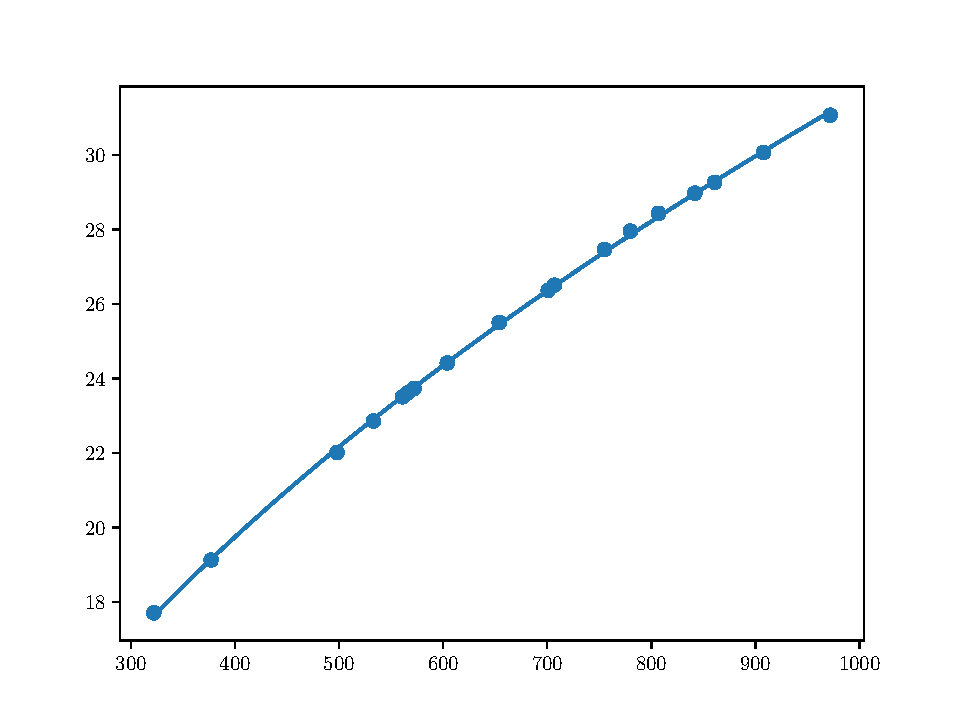
\includegraphics[scale=0.7]{lin.pdf}
    \end{center}
  \caption{Graf ukazující závistlost $t_{i}$ a $\sigma$}
\end{figure}
\newpage

\end{document}
